%导言区——进行全局设置
\documentclass{article} %有且仅有一个,可设置为article,book, report, letter

\usepackage{ctex}	%引入ctex宏包输出中文 编辑器中编码格式设置为UTF-8,编译器选择为XeLaTeX

% 导言区:\usepackage{graphicx}
% 语  法:\includegraphics[<选项>]{<文件名>}
% 格  式:EPS,PDF,PNG,JPEG,BMP

\usepackage{graphicx}
\graphicspath{{figures/},{pics/}} %图片的搜索路径在当前路径下的figures文件夹或pics文件夹中

\begin{document}
	\LaTeX 中的插图见图\ref{pic3}:
	
	%浮动体是为排版更紧密,可使图片不必放在正文下面,避免页面留白
	\begin{figure}[htbp] %[htbp]是指定浮动体的允许排版位置,h此处here、t页顶top、b页底bottom、p独立一页page,htbp就是允许各个位置
		\centering	%居中显示
		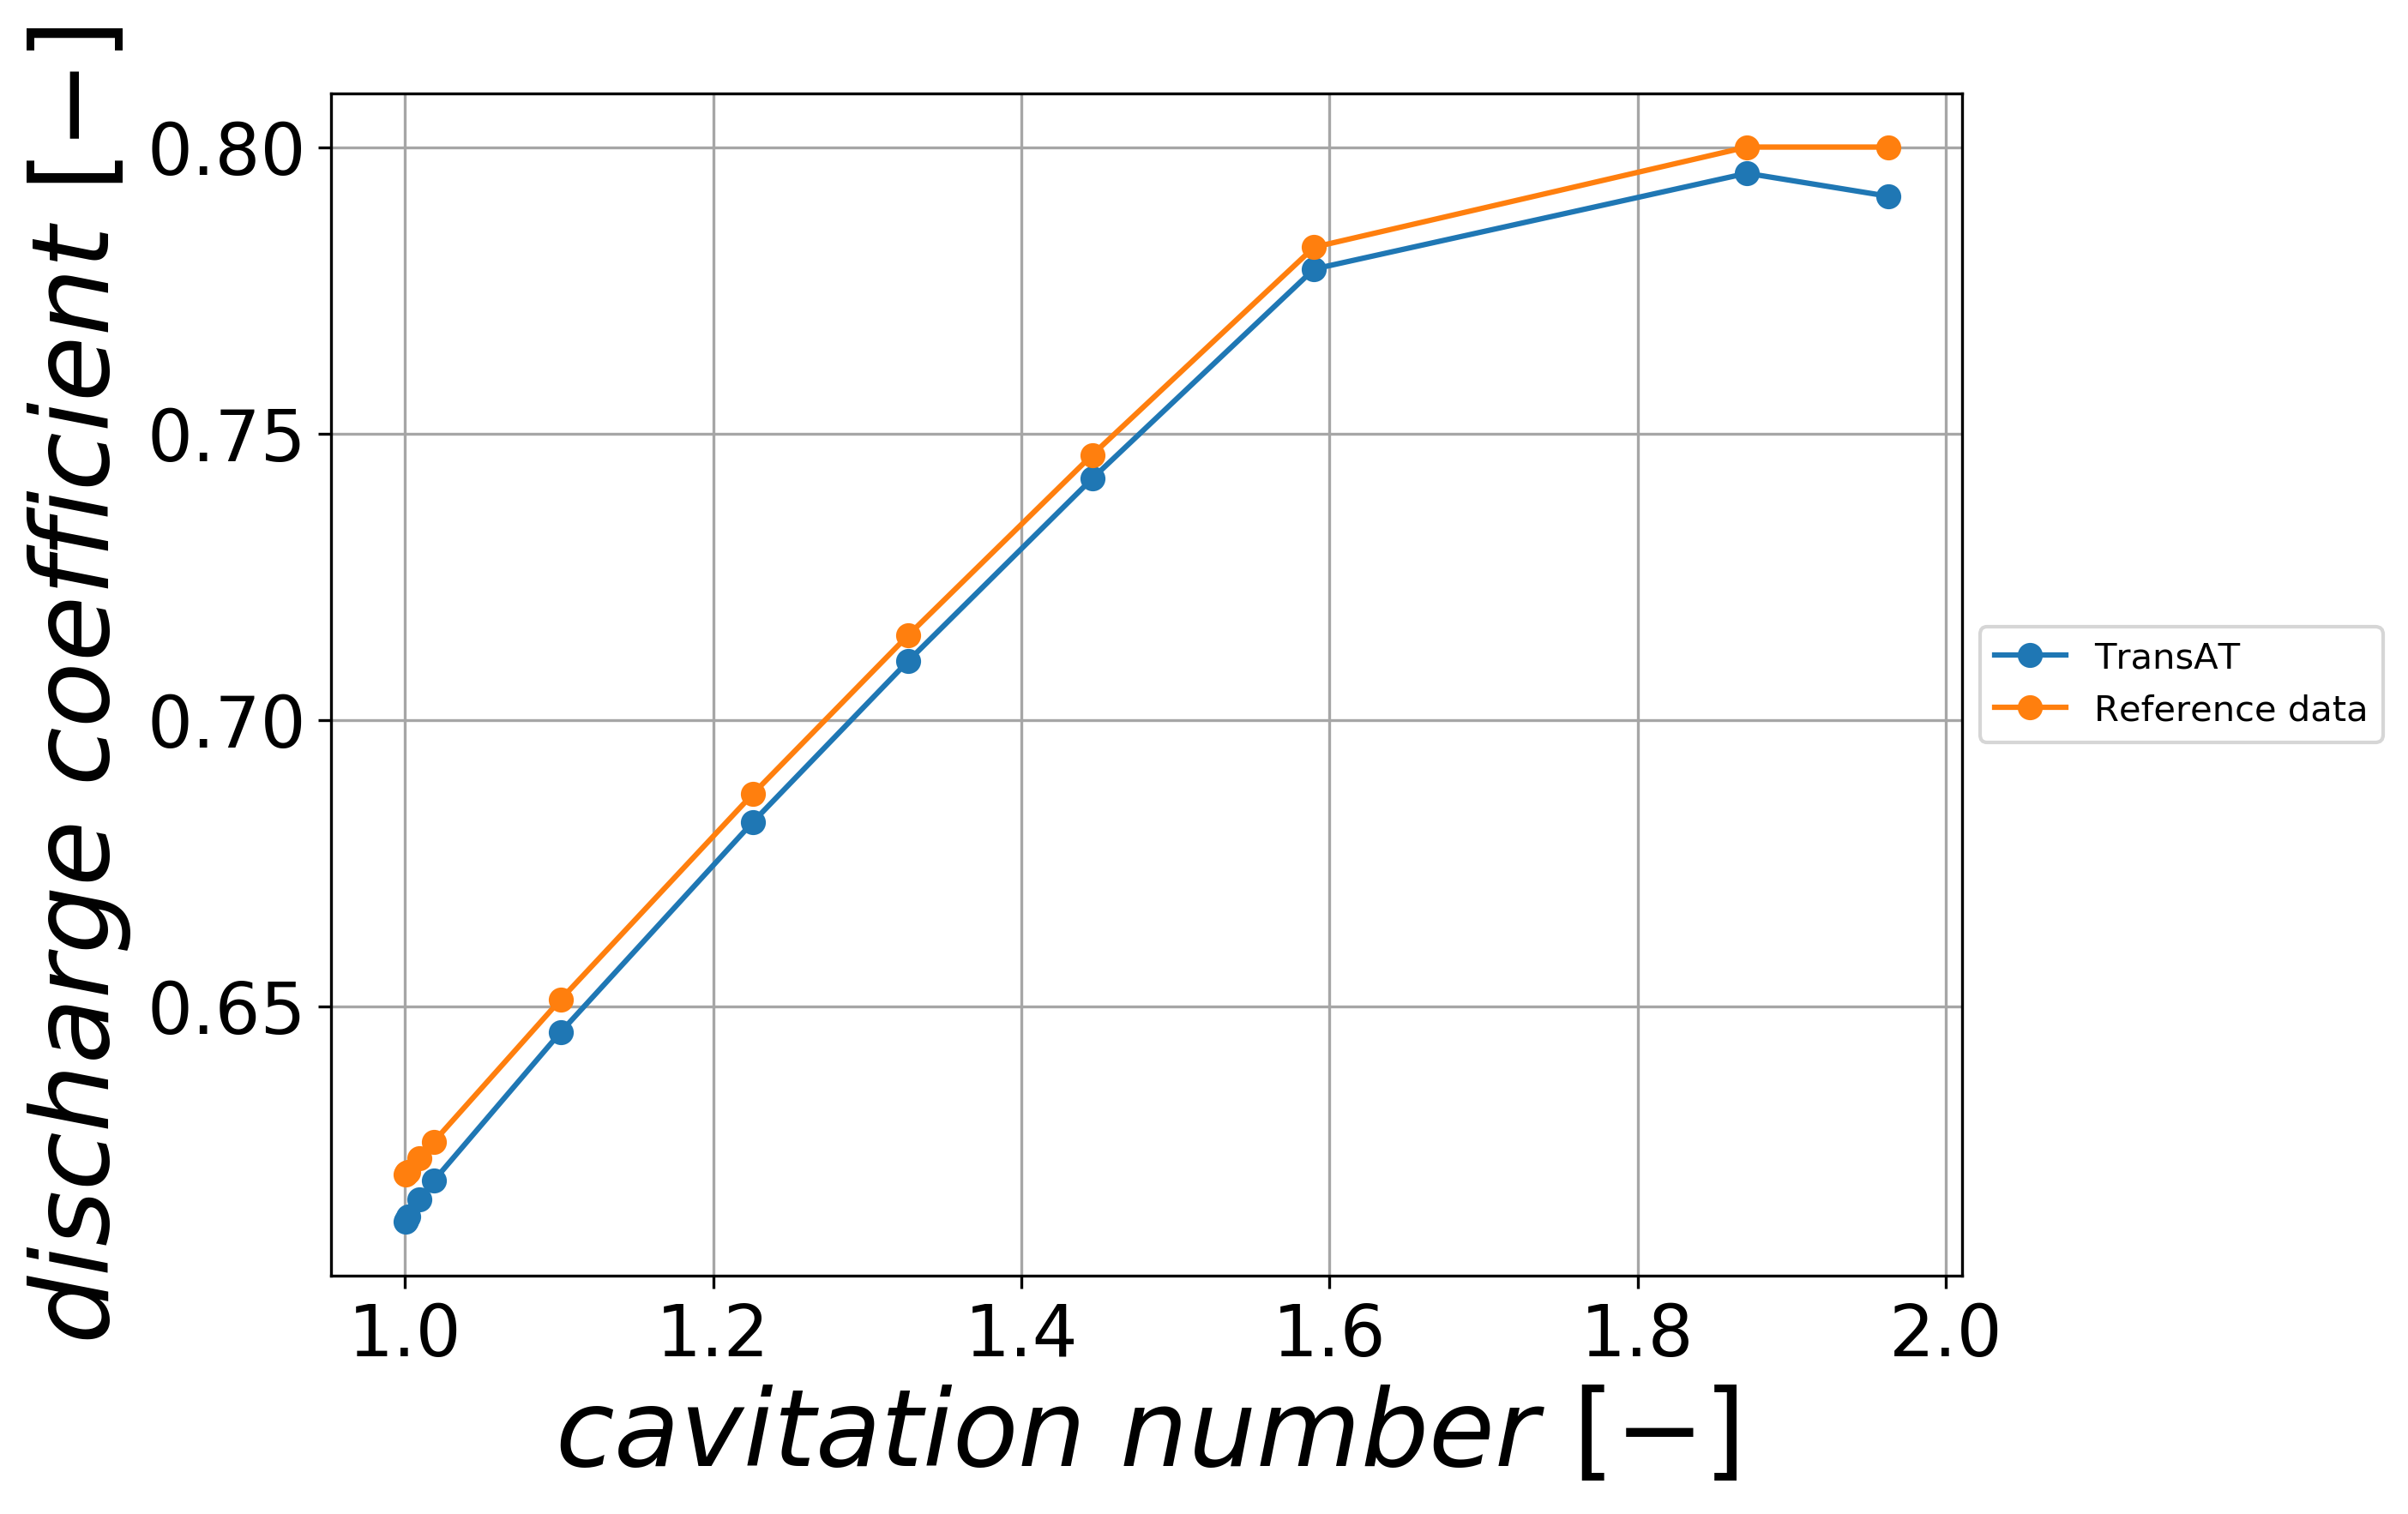
\includegraphics[scale=0.5]{3.png}
		\caption{系数分布}	%设置插图标题,会自动编号
		\label{pic3}	%\labe与\ref来实现交叉引用
	\end{figure}
\end{document}